\documentclass{article}
\usepackage{tikz-qtree}
\usepackage{fullpage}
\usepackage{booktabs}
\usepackage{amsmath}
\usepackage{amssymb}
\usepackage[noend]{algorithmic}
\usepackage[nothing]{algorithm}
\usepackage{tikz}
\usepackage{latexsym}
\usepackage{float}
\usepackage{hyperref}
\usetikzlibrary{arrows,automata}
\providecommand{\e}[1]{\ensuremath{\times 10^{#1}}}
\renewcommand{\thealgorithm}{}
\renewcommand*{\thefootnote}{[\arabic{footnote}]}
\title{CS 550: Programming Languages \\ Final}
\author{Dustin Ingram}
\begin{document}
\maketitle
\section{Grammars, Attributes, and Ambiguity}
\begin{enumerate}
    \item \textbf{Solution:} There are two possible derivations for
    \texttt{car([])}: \\
    \begin{center}
    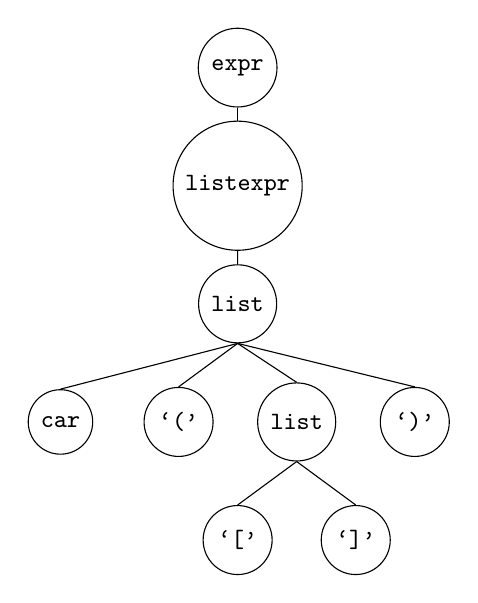
\begin{tikzpicture}
        \tikzstyle{every node}=[circle,draw,font=\small]
        \node {\texttt{expr}}
            child { node {\texttt{listexpr} }
                child { node {\texttt{list}}
                    child { node {\texttt{car}}}
                    child { node {\texttt{`('}}}
                    child { node {\texttt{list}}
                        child { node {\texttt{`['}}}
                        child { node {\texttt{`]'}}}
                    }
                    child { node {\texttt{`)'}}}
                }
             }
        ;
    \end{tikzpicture}
    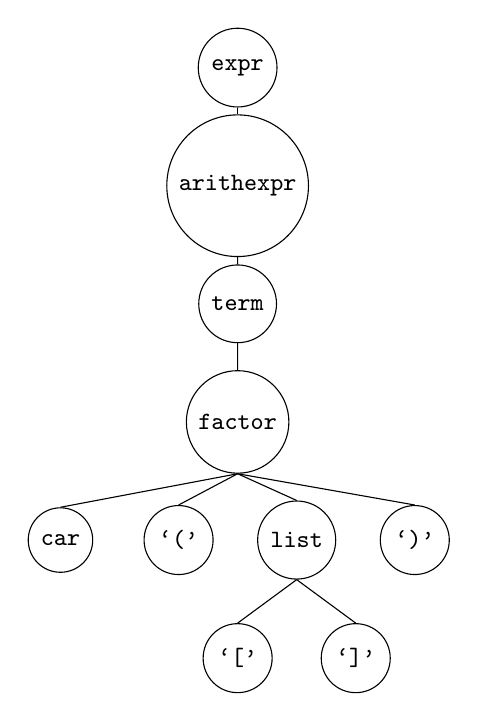
\begin{tikzpicture}
        \tikzstyle{every node}=[circle,draw,font=\small]
        \node {\texttt{expr}}
            child { node {\texttt{arithexpr} }
                child { node {\texttt{term}}
                    child { node {\texttt{factor}}
                        child { node {\texttt{car}}}
                        child { node {\texttt{`('}}}
                        child { node {\texttt{list}}
                            child { node {\texttt{`['}}}
                            child { node {\texttt{`]'}}}
                        }
                        child { node {\texttt{`)'}}}
                    }
                }
             }
        ;
    \end{tikzpicture}
    \end{center}
    \item \textbf{Solution:} \\ \\
    \begin{tabular}{l l}
        FIRST: & \\
        \hline
        \texttt{P} &      \texttt{atom, `, (} \\
        \texttt{E} &      \texttt{atom, `, (} \\
        \texttt{Es} &     \texttt{atom, `, (} \\
        & \\
        & \\
        & \\
        & \\
        & \\
    \end{tabular}
    \begin{tabular}{l l}
        FOLLOW: & \\
        \hline
        \texttt{P}   &    $none$ \\
        \texttt{E}   &    \texttt{atom, `, (, ), \$\$} \\
        \texttt{Es}  &    \texttt{)} \\
        \$\$ & $none$ \\
        \texttt{atom} & \texttt{atom, `, (, \$\$} \\
        \texttt{`} & \texttt{atom, `, (} \\
        \texttt{(} & \texttt{atom, `, (} \\
        \texttt{)} & \texttt{atom, `, (, ), \$\$} \\
    \end{tabular}
    \begin{tabular}{l l}
        PREDICT: & \\
        \hline
        \texttt{P $\to$ E \$\$}  &              \texttt{atom, `, (} \\
        \texttt{E $\to$ atom}   &             \texttt{atom} \\
        \texttt{E $\to$ ` E}     &    \texttt{`} \\
        \texttt{E $\to$ ( E Es )} &   \texttt{(} \\
        \texttt{Es $\to$ E Es}    &   \texttt{atom, `, (} \\
        \texttt{Es $\to$ $\varepsilon$}       &   \texttt{)} \\
        & \\
        & \\
    \end{tabular}
\end{enumerate}
\section{Mini Language Interpreter} The program data structure is as follows: \\
    \begin{center}
    \begin{tikzpicture}[
    level 2/.style={sibling distance=50mm},
    level 3/.style={sibling distance=15mm},
    level 7/.style={sibling distance=30mm},
    level 8/.style={sibling distance=15mm},
    level distance=10mm]
    \tikzstyle{every node}=[font=\footnotesize]
        \node {\texttt{program}}
            child { node {\texttt{stmt\_list} }
                child { node {\texttt{stmt}}
                    child { node {\texttt{define\_stmt}}
                        child { node {$addr$}}
                        child { node {\texttt{param\_list}}
                            child { node {$n$}}
                        }
                        child { node {\texttt{stmt\_list}}
                        child { node {\texttt{stmt}}
                        child { node {\texttt{if\_stmt}}
                        child { node {\texttt{expr}}
                            child { node {\texttt{term}}
                            child { node {\texttt{factor}}
                            child { node {$n$}}
}
}
}
                            child { node {\texttt{stmt\_list}}
                            child { node {\texttt{stmt}}
                            child { node {\texttt{assign\_stmt}}
                            child { node {$return$}
}
                            child { node {\texttt{expr}}
                            child { node {\texttt{expr}}
                            child { node {\texttt{term}}
                            child { node {\texttt{factor}}
                            child { node {$n$}
}
}
}
}
                            child { node {\texttt{term}}
                            child { node {\texttt{factor}}
                            child { node {\texttt{funcall}}
                            child { node {$addr$}
}
                            child { node {\texttt{expr\_list}}
                            child { node {\texttt{expr}}
                            child { node {\texttt{expr}}
                            child { node {\texttt{term}}
                            child { node {\texttt{factor}}
                            child { node {$n$}
}
}
}
}
                            child { node {\texttt{term}}
                            child { node {\texttt{factor}}
                            child { node {1}
}
}
}
}
}
}
}
}
}
}
}
}
                            child { node {\texttt{stmt\_list}}
                            child { node {\texttt{stmt}}
                            child { node {\texttt{assign\_stmt}}
                            child { node {$return$}}
}
                            child { node {\texttt{expr}}
                            child { node {\texttt{term}}
                            child { node {\texttt{factor}}
                            child { node {0}
}
}
}
}
}
}
}
}
}
                    }
                }
                child { node {\texttt{stmt}}
                    child { node {\texttt{assign\_stmt}}
                        child { node {$n$}}
                        child { node {\texttt{expr}}
                            child { node {\texttt{term}}
                            child { node {\texttt{factor}}
                            child { node {5}}
}
}
}
                        }
                }
                child { node {\texttt{stmt}}
                child { node {\texttt{assign\_stmt}}
                child { node {5}}
                child { node {\texttt{expr}}
                child { node {\texttt{term}}
                child { node {\texttt{factor}}
                child { node {\texttt{funcall}}
                child { node {$addr$}}
                child { node {\texttt{expr\_list}}
                child { node {\texttt{expr}}
                child { node {\texttt{term}}
                child { node {\texttt{factor}}
                child { node {$n$}}
}
}
}
}
}
}
}
}
}
}
             }
        ;
    \end{tikzpicture}
    \end{center}
    As the \texttt{eval} method for the program object is called, this program structure is built and the environment is modified accordingly, as the \texttt{eval} method is then called on each child object, until the leaves are reached. The resulting environment is: \\
\begin{center}
\begin{tabular}{l l}
ENV: & \\
\hline
\texttt{addr} &  $procedure$    \\
\texttt{n} &  5    \\
\texttt{s} &   15  \\
\texttt{return} & 15 \\
\end{tabular}
\end{center}

    \section{Shift Reduce Parsing and Parser Generation}
    \begin{enumerate}
        \item \textbf{Solution:}
    \begin{center}
    \begin{tabular}{l l l}
\multicolumn{2}{l}{CSFM for the Grammar:} & \\
\hline
0. &  list $\to$ $\bullet$(        &       on ( shift and goto 2\\
& & \\
1. &  list $\to$ ($\bullet$(        &      on ( shift and goto 1\\
  &  list $\to$ ($\bullet$)          &    on ) shift and reduce (pop 1 state, push list on input)\\
  &  list $\to$ ($\bullet$sequence    &       on sequence shift and goto 6\\
  &  list $\to$ ($\bullet$number       &      on number shift and reduce (pop 1 state, push list on input)\\
  &  list $\to$ ($\bullet$list          &     on list shift and reduce (pop 2 states, push list on input)\\
  &  list $\to$ ($\bullet$listelement    &        on listelement shift and goto 4\\
& & \\
2. &  list $\to$ ($\bullet$)     &         on ) shift and reduce (pop 1 state, push list on input)\\
  &  list $\to$ ($\bullet$(       &       on ( shift and goto 1\\
  &  list $\to$ ($\bullet$sequence &          on sequence shift and goto 3\\
  &  list $\to$ ($\bullet$number    &         on number shift and reduce (pop 1 state, push list on input)\\
  &  list $\to$ ($\bullet$listelement&            on listelement shift and goto 4\\
  &  list $\to$ ($\bullet$list        &       on list shift and reduce (pop 2 states, push list on input)\\
& & \\
3. &  list $\to$ ( sequence$\bullet$)  &           on ) shift and reduce (pop 2 states, push list on input)\\
& & \\
4. &  sequence $\to$ (listelement$\bullet$,&       on , shift and goto 5\\
  &  sequence $\to$ (listelement$\bullet$)  &     on ) shift and reduce (pop 2 state, push sequence on input)\\
& & \\
5 .&  sequence $\to$ (listelement,$\bullet$sequence &  on sequence shift and reduce (pop 1 state, push sequence on input)\\
  &  sequence $\to$ (listelement,$\bullet$number   &  on number shift and reduce (pop 1 state, push sequence on input)\\
  &  sequence $\to$ (listelement,$\bullet$listelement&    on listelement shift and goto 4\\
  &  sequence $\to$ (listelement,$\bullet$list  &     on list shift and reduce (pop 2 states, push list on input)\\
  &  sequence $\to$ (listelement,$\bullet$(  &    on ( shift and goto 1\\
& & \\
6. &  list $\to$ (sequence$\bullet$)    &      on ) shift and reduce (pop 2 states, push list on input)\\
\end{tabular}
\end{center}
    \item \textbf{Solution:}
    \begin{center}
    \begin{tabular}{l l l}
Parse stack & Input stream & Comment \\
\hline
0 & (1, (2)) & \\
0 ( & 1, (2)) & on ( shift and goto 2 \\
0 ( $number$ & , (2)) & on number shift and reduce \\
0 ( $number$, & (2)) & on , shift and goto 5 \\
0 ( $number$, ( & 2)) & on ( shift and goto 1 \\
0 ( $number$, ( $number$ & )) & on number shift and reduce\\
0 ( $number$, ( $number$ ) & ) & on ) shift and reduce\\
0 ( $number$, ( $number$ ) ) & & on ) shift and reduce\\
done & & \\
\end{tabular}
\end{center}
\end{enumerate}
\section{Mini Language Compiler}
\begin{enumerate}
    \item \textbf{Solution:}
\begin{center}
\begin{verbatim}
A: Code(stmt-list)
 : Code(expr)
 : LD t
 : JMZ B 
 : JMP A
B: ...
\end{verbatim}
\end{center}
    \item \textbf{Solution:}
\begin{center}
\begin{tabular}{l l}
Activation Record: & \\
\hline
Parameters: &  $n = 3$ \\
Local Variables: & \\
Temporary Variables: & T1, \dots , T6 \\
Return Value: &    6 \\
Previous Frame Pointer: &  10 \\
Return Address: &  50 \\
\end{tabular}
\end{center}

\end{enumerate}
\section{Dynamic Memory Allocation and Garbage Collection}
\begin{enumerate}
    \item \textbf{Solution:} $L = ( (2, 3), ( ) )$
    \item \textbf{Solution:} $Available = 0 = (0, 1, 5, 6)$
\end{enumerate}
\section{Dynamic Arrays}
\begin{enumerate}
    \item \textbf{Solution:} Changes to the grammar:  \texttt{expr $\to$ IDENT `[' expr `]' } \\ New classes: \texttt{CreateArray} and \texttt{DeleteArray} for the \texttt{array} and \texttt{delete} functions, and an \texttt{Array} class for the array.
    \item \textbf{Solution:}
        The \texttt{eval} method of \texttt{CreateArray} allocates a new \texttt{Array} object with $n$ elements, using available memory cells. 

The \texttt{eval} method of \texttt{DeleteArray}, marking it's respective memory cells as free. 

The \texttt{eval} method of \texttt{Array} would look up the corresponding Identifier, then return the value for the index provided.
    \item \textbf{Solution:}
        The \texttt{CreateArray} function must validate that the array size is a positive integer and that there is sufficient memory to create it.

The \texttt{DeleteArray} function must validate that it has been passed an existing \texttt{Array}

The \texttt{Array} function must validate that the identifier is valid, and that the index is a positive integer and that it is within the bounds of the array.

\end{enumerate}
\end{document}
